%----------------------------------------------------------------------------------------
%----------------------------------------------------------------------------------------
%----------------------------------------------------------------------------------------
%DATA
%----------------------------------------------------------------------------------------
%----------------------------------------------------------------------------------------
%----------------------------------------------------------------------------------------

\section{DATA}
\label{sec: data}
%Basically these are 2012 data
As mentioned in Sec.~\ref{sec: intro}, for training neural networks, we used SED templates from K96. % PB160426: don't need the "as mentioned in Sec" since this is the paragraph right after it. 
Moreover, to test our networks, we obtained SED and physical properties of 142 galaxies at 0.5 < $z$ < 1 from T12.
 \subsection{Kinney spectral model}
     \begin{figure}
        \centering
        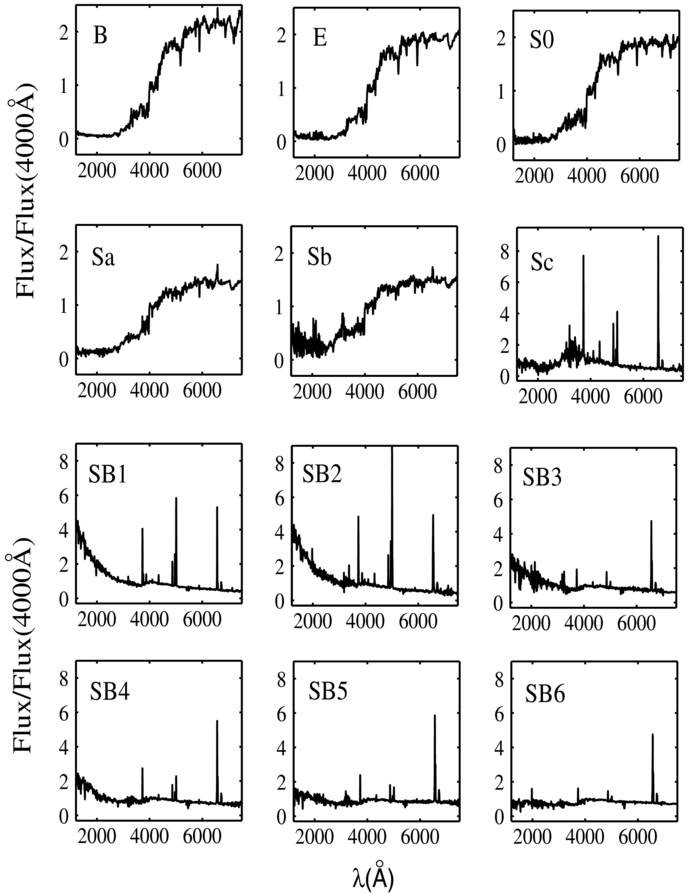
\includegraphics[width=0.5\textwidth]{../images/k96.jpg}
        \caption{K96 spectra template for 12 types of galaxies from T12 paper.Type of each template is shown in each frame. Plots B, E, S0, Sa, Sb and SC show spectra that belongs to early type galaxies. Star burst galaxies spectra are indicated with SB 1 to 6. Higher numbers represents more inartistic colour extinction.}
        \label{fig: k96}
    \end{figure}
    K96 produced a template of UV-optical spectra of 70 star forming and quiescent galaxies which can be used to classify the SED of the high redshift galaxies. % PB160426: they produced 70 templates, or they used 70 spectra to produce templates? Also, I think you need some stronger arguments for why K96 is a good set of templates to use. Nothing better developed in the last 20 years? Do they span the whole range of properties you expect the 0.5<z<1.0 galaxies to have?
    They introduced 12 types of spectra based on their morphological type or colour excess for quiescent and star burst galaxies, respectively (Fig.~\ref{fig: k96}). % PB160426: I'd use 'extinction' rather than 'colour excess' here and elsewhere.
    %I know it is exactly as Hossein's plot, but I can see any other choice to put here. % PB160426: I think that's OK, but you will need to look up the journal rules for reproducing a figure from another paper.

    The quiescent group of galaxies includes Elliptical (E), Bulge (B), S0, Sa, Sb, and Sc galaxies.
    Bulge groups represents galaxies similar to M31 and M81, which their UV and optical spectroscopy dominated by the stellar population in their bulges.
    
    The star burst galaxies are divided in six groups (SB1 - SB6) based on their inartistic colour extinctions ($E(B-V)$). 
    As it is clear in the Fig.~\ref{fig: k96}, SB1 galaxies have lower internal colour excess ($E(B-V) \simeq 0.05$) while SB6 galaxies have the highest amount of extinction ($E(B-V) \simeq 0.65$) among star burst galaxies.
    
    K96 spectra spans from $\sim1200-1000$\AA. % PB160426: that's rest frame right? Should 1000 be 10000?
    However, we only used data between $\sim1200-1000$\AA~in Fig.~\ref{fig: k96}, over availability of flux information in those wavelength for all 12 groups.
    In early type galaxies spectrum (B-Sb), spectra is redder and strong absorption lines, and 4000\AA~break is distinguishable. 
    While SEDs of star burst galaxies are more flatter than early type one and show strong emission lines.
    For more details on each spectra type, we encourage readers to see K96 and references therein. 
    

 \subsection{SED and Properties of the sample galaxies}
    T12 selected 142 galaxies from the spectroscopic campaign of the ESO GOODS-South field, which have a photometry data from the Good-MUSIC catalogue. % PB160426: *how* were the galaxies selected? Why 142?
    The photometry data contains data in 10 - 13 filters with wavelength range of $\sim 0.4-24 \mu$m. % PB160426:rest-frame or observed frame? I assume these galaxies have spectroscopic redshifts, or were redshifts derived from photometry?
    They used these photometry data as inputs for Code Investigating GALaxy Emission ({\em CIGALE} code;~\citep{Noll09}) to generate the best fitted SED for each galaxy as well as some of the physical properties of the galaxies.
    
    {\em CIGALE} is a valuable tool to investigate the properties of the galaxy using UV to IR wavebands.
    It uses stellar populations, synthetic attenuation and dust emission models, spectral line templates, and active galactic nuclei's optical spectral templates to model SED of the galaxies.
    This code were successfully tested with data from 39 galaxies selected from the Spitzer Infrared Nearby Galaxy Survey (SINGS;~\citep{Kennicutt03}) by N09.
    T12 produced the best SED match for each galaxies.
    For testing the created networks, we only used part of the spectra that have the same wavelength as K96 SEDs. %PB160427: need to be more explicit here about exactly what the spectra being analyzed are. Is the data vector for each object a list of fluxes (flux densities) as a function of (rest) wavelength? Same wavelengths for every object? What is the spectral resolution? Do the spectra include the whole galaxy or just the cental part?
    Then, they used an exponentially decreasing SFR, visual attenuation ($\tau$) model and derived physical properties of galaxies such as age, and stellar mass.
    Some of these properties are shown in Tab~\ref{tab: props}.
    In the Sec.~\ref{sec: 1D}, we studied these properties for each categorization. % PB160426: this paragraph seems to have "what they did" and "what we did" mixed up -- makes more sense to separate?
    They assumed the Salpeter initial mass function~\citep{Salpeter55} and old stellar population age of $\sim 10$~Gyr.
    More details on creating SEDs and extracting information about galaxies properties using {\em CIGALE} can be found in N09 and T12.
    
    \begin{table}
\caption[]{Description of the properties of T12 galaxies; the output result of {\em CIGALE}}     
\label{tab: props}
\centering
\begin{tabular}{l l l}
\hline\hline
\noalign{\smallskip}
Par. & Unit & Description\\
\noalign{\smallskip}
\hline
\noalign{\smallskip}
$t_{\,\mathrm{oSP}}$ & Gyr & age of old SP model \\
$t_{\,\mathrm{ySP}}$ & Gyr & age of young SP model \\
$f_\mathrm{burst}$ & --- & mass fraction of \\
& & young single population (SP) model \\
\noalign{\smallskip}
$t_{\,\mathrm{D4000}}$ & Gyr & D4000-related age. \\
\noalign{\smallskip}
$M_\mathrm{star}$ & M$_\odot$ & total stellar mass  \\
SFR & M$_\odot$/yr & instantaneous SFR  \\
$A_\mathrm{FUV}$ & mag & attenuation at 1500\,\AA{} \\
\noalign{\smallskip}
\hline
\end{tabular}
\end{table}
